\section{Pipeline}

\tikzstyle{process} = [rectangle, rounded corners, minimum width=2cm, minimum height=1cm,text centered, draw=black, fill=gray!50]

\begin{figure}[h]
    \centering
    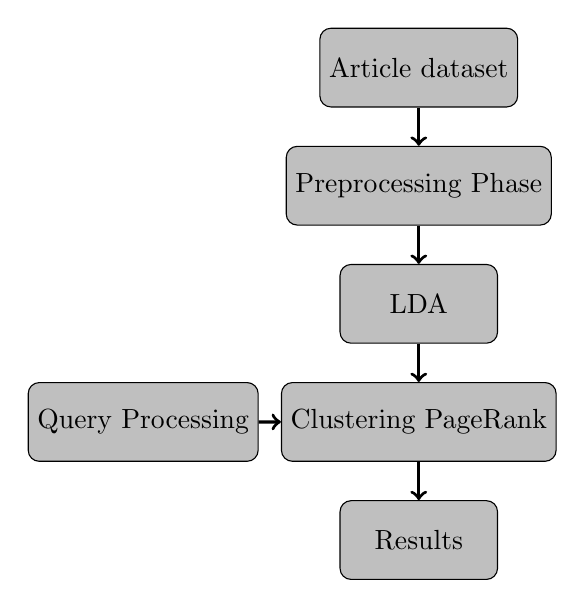
\begin{tikzpicture}[node distance=1.5cm]
    %\draw[step=1cm,gray,very thin] (-8,-8) grid (8,8);
	\node (Dataset) [process] {Article dataset};
	\node (Cleaning)[process, below of=Dataset] {Preprocessing Phase};
	\node (Training) [process, below of=Cleaning] {LDA};
	\node (Cluster PR) [process, below of=Training] {Clustering PageRank};
	\node (Query) at (-3.5, -4.5) [process] {Query Processing};
	\node (Result) [process, below of=Cluster PR] {Results};
	\draw [->, very thick] (Dataset) edge (Cleaning); 
	\draw [->, very thick] (Cleaning) edge (Training);
	\draw [->, very thick] (Training) edge (Cluster PR);
	\draw [->, very thick] (Cluster PR) edge (Result);
	\draw [->, very thick] (Query) edge (Cluster PR);
\end{tikzpicture}
	\caption{Pipeline}
    \label{fig:pipeline}
\end{figure}
The pipeline of our framework is divided into five different phases which are displayed in \autoref{fig:pipeline}.

\subsection{Article dataset}
We have an dataset consisting of articles from the media group Nordjyske, whose primary focus is maintaining a variety of local newspapers within the North Jutland region of Denmark. 
The data is from 2017-2019, where a total of ~270.000 articles have been extracted from their database.

\subsection{Preprocessing}
The articles are on the format:
\begin{itemize}
	\item Id
	\item Headline
	\item Body
\end{itemize}
When training the LDA model, we concatenate the Headline and Body for simplicity.
The preprocessing phase is described further in detail in \todo[inline]{ref til preprocessing}.
This phase applies some processes to simplify the dataset and remove redundant noise from the data. 
After the preprocessing phase, we are left with 130.000 articles.

\subsection{LDA}
We apply the \acrfull{LDA} to the dataset in order to generate topic clusters based on the content of the articles. 
We detail the investigation and selection of hyper parameters in \todo{ref til LDA section}. 
After the model has been trained, we use the topic distributions as clusters in the next phase.

\subsection{Clustering PageRank}
In this phase, we apply a clustering random walk to the articles and the clusters given in the \gls{LDA} phase, and this phase yields a prioritized list of articles based on the query provided.


\subsection{Query Processing}



